\pgfsetplotmarksize{0pt}
\begin{figure}
 \centering
 \caption{\label{fl_conv3}FLClustered/test3.txt},
 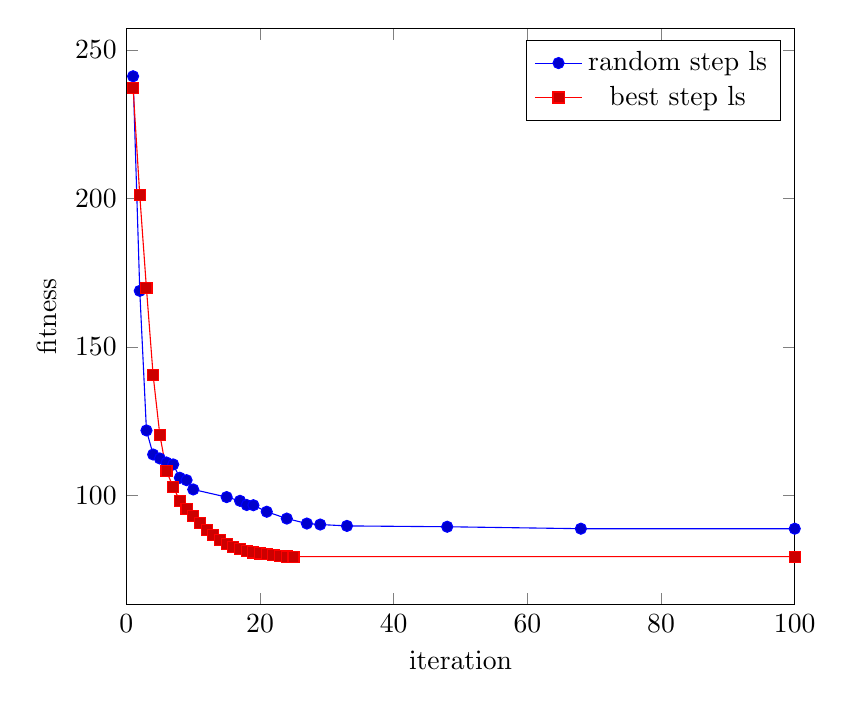
\begin{tikzpicture}
 \begin{axis}[
   width=0.7\textwidth,
   scale only axis,
   xlabel=iteration,
   ylabel=fitness,
   xmin=0,xmax=100,
   domain=0:100]
   \addplot coordinates {
     (0,inf)
     (1,241.098)
     (2,168.863)
     (3,121.88)
     (4,113.782)
     (5,112.447)
     (6,111.081)
     (7,110.441)
     (8,105.942)
     (9,105.137)
     (10,102.012)
     (15,99.4384)
     (17,98.1855)
     (18,96.7847)
     (19,96.7098)
     (21,94.5151)
     (24,92.2122)
     (27,90.5451)
     (29,90.206)
     (33,89.7439)
     (48,89.4609)
     (68,88.8051)
     (100,88.8051)
   };
   \addlegendentry{random step ls}
   \addplot coordinates {
     (0,inf)
     (1,237.166)
     (2,201.008)
     (3,169.693)
     (4,140.431)
     (5,120.424)
     (6,108.159)
     (7,102.845)
     (8,98.2332)
     (9,95.5011)
     (10,93.0335)
     (11,90.6819)
     (12,88.4615)
     (13,86.6378)
     (14,85.0514)
     (15,83.5191)
     (16,82.6186)
     (17,81.9829)
     (18,81.3728)
     (19,80.8136)
     (20,80.4713)
     (21,80.1764)
     (22,79.8598)
     (23,79.5761)
     (24,79.4294)
     (25,79.4056)
     (100,79.4056)
   };
   \addlegendentry{best step ls}
 \end{axis}
 \end{tikzpicture}
\end{figure}
